\section{Line of Sight Depths}
\label{891_2:sec:LOS}

\begin{figure*}
  \centering
  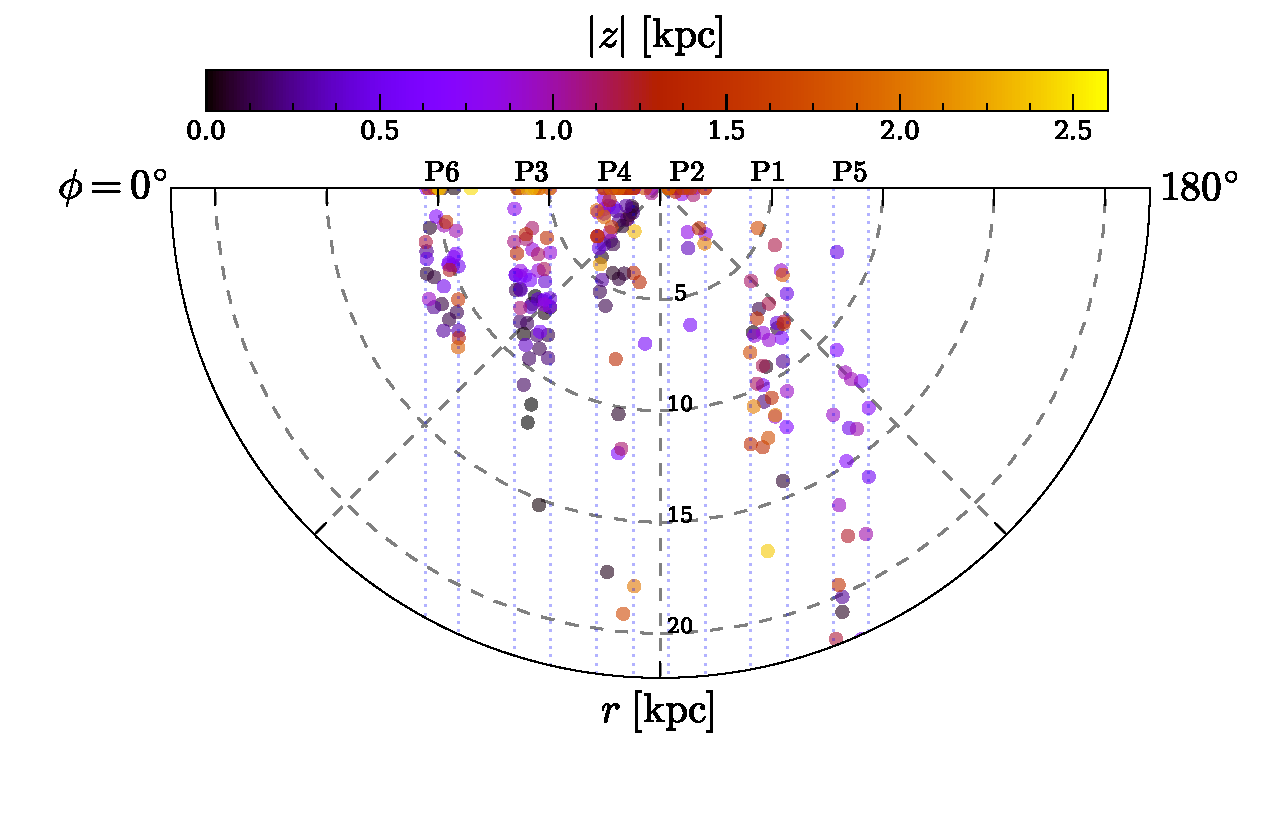
\includegraphics[width=0.9\textwidth, trim={0 1.5cm 0 0}, clip]{891_2/figs/velocity_projection.pdf}
  \caption[Map of \GP apertures in cylindrical
    coordinates]{\fixspacing\label{891_2:fig:velocity_projection}Map
    of the physical location of average emission from each aperture,
    as determined by a velocity-based LOS depth calculation (equations
    \ref{891_2:eq:vel_LOS}). The vertical dotted lines show the
    boundaries of the \GP pointings described in \ref{chap:891_1}.}
\end{figure*}

To report our quantities of interest as a function of height and true,
galactic radius we need to deproject our measured radii into radii
with respect to the true center of NGC 891. This deprojection relies
on understanding the average line-of-sight (LOS) depth to the emitting
material in each \GP aperture. This LOS depth can be computed from the
measured tangential velocity in each aperture.

In the absence of any attenuating material (i.e., dust) the maximum
velocity measured in each aperture will be the tangential speed of the
galaxy at any given radius and height, which, to first order is well
approximated by the circular speed of the galaxy.  In reality,
however, when looking through an edge-on disk with high attenutation
the measured velocity is the projected velocity of emitting material
along the entire sight-line, which will become opaque before reaching
the tangent point. Thus, by comparing the measured velocity to the
known circular velocity at a given radius we can determine the LOS
depth to the emitting material.

Under the assumption that all material in the galaxy rotates at the
circular speed the relation between measured and circular velocity
comes from simple geometry. Given a measured projected radius and
velocity, $r_{\mathrm{proj}}$ and $V_{\mathrm{obs}}$, respectively,
the effective location of the emitting material in cylindrical
coordinates centered on galaxy is
\begin{align}
  \label{891_2:eq:vel_LOS}
  \phi &= \cos^{-1}\left(\frac{V_{\mathrm{obs}}}{V_{\mathrm{c}}}\right)\\
  r &= r_{\mathrm{proj}}\frac{V_{\mathrm{c}}}{V_{\mathrm{obs}}},
\end{align}
where $V_{\mathrm{c}}$ is the circular velocity. Due to the nearly
perfect edge-on nature of NGC 891 the projected radius,
$r_\mathrm{proj}$, can be measured directly as the on-sky distance
from the galaxy center. Measurements of $V_\mathrm{obs}$ are described
in \S\ref{891_2:sec:vel}.

To compute $V_c$ we construct a simple model rotation curve using
circular velocities derived from envelop-fitting the HI data of
\citet{Swaters97}. We also include the height-dependence on cicular
speed reported by \citet{Oosterloo07}. These measurements of the
circular speed are based on collisional particles (i.e., gas) and are
therefore not perfect estimates for the circular speed of the stars,
which will lag the gas slightly due to assymetric drift, but in the
absence of measurements of the true, stellar circular speed the gas
velocities make an acceptable approximation. Our rotation curve for
NGC 891 is thus
\begin{multline}
  V_{\mathrm{c}}(r_{\mathrm{proj}},z) =
  (\val{-15.79}{\kms})\left(\frac{z}{\mathrm{kpc}}\right) \\ 
  + \left\{
    \begin{array}{ll}
      (\val{68.2}{\kms})\left(\frac{r_{\mathrm{proj}}}{\mathrm{kpc}}\right)
      & r_{\mathrm{proj}} < \val{3.3}{kpc}\\ \val{225}{\kms} &
      r_{\mathrm{proj}} \geq \val{3.3}{kpc}.\\
    \end{array}
    \right.
\end{multline}

%+++++++++++++++++++=
%% {\bf MAB: Note sentence I broke out about HI measuing circular
%%   speed. This needs a reference and also discussion up front of how
%%   you are going to use the measured variation in this speed with
%%   height from Oosterloo07. This should be noted again in the sentence
%%   starting with the sentnece ``Under the assumption...'' You can still
%%   leave your model to the end of the par. More broadly you want to
%%   discuss whether the trends in HI tangential speed with height is
%%   representative of the potential or a lagging gas halo that may not
%%   reflect the stellar tangential speed. Similarly, you should not the
%%   amplitude of the rotation and the vertical correction relative to
%%   asymmetric drift. I think the point is that the model is not perfect
%%   for stars, but seems a reasonable approach to the best
%%   approximation. 
%------------------
%    You should discuss how uncertainties in the velocity
%%   model project to uncertainties in the inferred LOS depth, nothing
%%   that this is unlikely to introduce differential effects between the
%%   two halves of the galaxy.

%++++++++++++++++++=
%%   I am wondering about this sentence: ``In reality, however, when
%%   looking through an edge-on disk with high attenutation the measured
%%   velocity is the projected, LOS velocity of the emitting material at
%%   approximately 1 optical depth.'' Is this right and how to we
%%   reconcile it with the fact that we measure optical depths
%%   considerably greater than 1 in many lines of sight?

%++++++++++++++++=
%%   I would say something slightly different than `` we can determine
%%   the LOS depth to the emitting material.'' We are measuring a
%%   characteristic mean depth.
%++++++++++++++++
%%   Let me recommend that you simplify eqn 14. by specifying that r and
%%   z have units of kpc (you should go back and do the same for eqn. 11
%%   in the previous setion). Also note format of km s$^{-1}$.

%% }


Figure \ref{891_2:fig:velocity_projection} shows each aperture in its
velocity-derived cylindrical coordinate. We define the approaching
side of the galaxy ($r_\mathrm{proj} < 0$) to be at $\phi <
90^{\circ}$ and the receeding side to have $\phi > 90^{\circ}$. With
this view the large-scale structure of NGC 891 becomes clear;
sight-lines to the receeding side of NGC 891 prob the back of a spiral
arm, where \citet{Kamphuis07b} identifies a higher concentration of
dust, and as a result our measurements do not sample very far into the
disk. Conversely on the approaching side we see the leading edge of a
spiral arm, which has less dust due to ongoing star formation. On the
approaching side of the galaxy there is also a clear trend that we see
farther into the disk at larger heights, which is consistent with dust
occupying a disk with a surface density that decreases with height.

%+++++++++++++++++++
%% {\bf MAB: Explain your coordinate system in the sense of what $\phi$
%%   values correspond to approaching and receding sides. I think you can
%%   get away with the Kamphuis07 (a or b) ref here at least in terms of
%%   the spiral arm picture. What I am wondering about is if you want to
%%   address something about the phase-angle and pitch of the arms
%%   (qualitatively) in order to justify your picture here. 
%-----------
%    Also, for the
%%   last sentence concerning height, this is very difficult to see from
%%   Fig 5. Have you tried plotting $R_{proj}/R_{LOS}$ (where I think
%%   $R_{LOS}$ is your r in eqn 13) vs z, marking for approaching vs
%%   receding? Or maybe it should be $R_{LOS}/R_{proj} - 1$ vs z. }

% \subsection{Extinction-based LOS Calculations}
% We can also estimate the LOS depth based on the measured optical depth in each
% aperture. Under the massively simplifying assumption that all of the
% attenuating material in NGC 891 occupies a doubly-exponential disk we can
% calculate the extinction coefficient at any point in the galaxy:
% \begin{equation}
%   \kappa(r,\phi,z) = \kappa_{V}\rho_0\exp\left(-\frac{r}{h_r}-\frac{|z|}{h_z}\right),
% \end{equation}
% where $r$, $\phi$, and $z$ are cylindrical coordinates, $\rho_0$ is density of
% dust at $r=z=0$, and $h_r$ and $h_z$ are the dust scale length and scale
% height, respectively. The optical depth at a given projected radius,
% $r_{\mathrm{proj}}$, and LOS depth, $y$, is then
% \begin{equation}
%   \tau_V(r_{\mathrm{proj}},y,z) = \exp\left(-\frac{|z|}{h_z}\right)\rho_0\kappa_V\int_0^y \exp\left(-\frac{\sqrt{r_{\mathrm{proj}}^2 + y'^2}}{h_r}\right) d y'.
% \end{equation}
% For our analysis we use values of $h_z=\val{0.29}{kpc}$,
% $h_r=\val{7.68}{kpc}$, and $\rho_0\kappa_V = \val{1.47}{m^{-1}}$, all taken
% from \citet{xilouris99}. {\bf NOTE: CHECK THE VALUE OF $\rho_0\kappa_V$}.

% In practice we compute the $\tau_V$ integral numerically for a grid of $y$
% values and then find the value of $y$ that matches \tauV measured from SSP
% fitting (\S\ref{891_2:sec:SSP_modeling}). Figure \ref{891_2:fig:tau_projection} shows each
% aperture in its \tauV-derived cylindirical coordinate. Note that right now
% this looks pretty messed up; at the largest heights the implication is that we
% can see through the entire galaxy. Maybe this isn't so crazy at \val{2}{kpc},
% but in that case why do we still measured $\tauV > 1$?

% \begin{figure}
%   \centering
%   \includegraphics[width=\columnwidth]{891_2/figs/tau_projection.png}
%   \caption{\label{891_2:fig:tau_projection}Map of the physical location of average
%     emission from each aperture, as determined by a \tauV-based LOS depth
%     calculation. The vertical dotted lines show the boundaries of the \GP
%     pointings shown in Figure \ref{891_2:fig:pointings}. Using the simple galaxy
%     model described in the text we find that many of the apertures show
%     measured \tauV values far above what would be expected at larger
%     heights. {\bf We need to confirm we're using the correct values. Also,
%       what about clumpiness, etc.?}}
% \end{figure}


% tau_balm vs tau_cont compared to predictions from e.g. Charlot
% projected radius map from velocity vs projected radius map from A_V
